\documentclass[tikz,border=3pt]{standalone}
\usepackage[T1]{fontenc}
\usepackage[utf8]{inputenc}
\usepackage[english]{babel}
\usepackage{mathptmx}
\usepackage[scaled=0.92]{helvet}
\usepackage{amsmath,amssymb,textcomp}
\usetikzlibrary{positioning,arrows.meta}
\newcommand{\us}{\textmu s}
\begin{document}
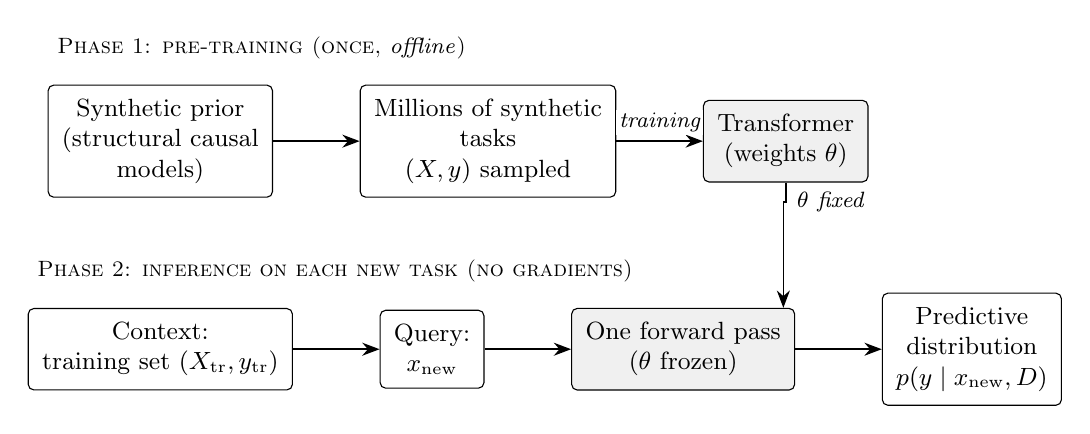
\begin{tikzpicture}[
  font=\small,
  caixa/.style={draw, rounded corners=2pt, align=center, inner sep=5pt,
                minimum height=9mm},
  destaque/.style={caixa, fill=black!6},
  rotulo/.style={font=\footnotesize\itshape, midway, fill=white,
                 inner sep=1pt},
  fase/.style={font=\footnotesize\scshape},
  seta/.style={-{Stealth[length=2.2mm]}, semithick},
  node distance=7mm and 11mm]

% Phase 1: pre-training
\node[caixa] (prior) {Synthetic prior\\(structural causal\\models)};
\node[caixa, right=of prior] (tarefas) {Millions of synthetic\\tasks\\
  $(X, y)$ sampled};
\node[destaque, right=of tarefas] (modelo) {Transformer\\(weights $\theta$)};
\node[fase, above=2mm of prior.north west, anchor=south west]
  {Phase 1: pre-training (once, \emph{offline})};

% Phase 2: inference
\node[caixa, below=14mm of prior] (contexto)
  {Context:\\training set $(X_{\text{tr}}, y_{\text{tr}})$};
\node[caixa, right=of contexto] (consulta)
  {Query:\\$x_{\text{new}}$};
\node[destaque, right=of consulta] (forward)
  {One forward pass\\($\theta$ frozen)};
\node[caixa, right=of forward] (pred)
  {Predictive\\distribution\\$p(y \mid x_{\text{new}}, D)$};
\node[fase, above=2mm of contexto.north west, anchor=south west]
  {Phase 2: inference on each new task (no gradients)};

\draw[seta] (prior) -- (tarefas);
\draw[seta] (tarefas) -- node[rotulo, above=2pt] {training} (modelo);
\draw[seta] (modelo.south) -- ++(0,-2.5mm) -| node[rotulo, pos=0.08, right=3pt]
  {$\theta$ fixed} ([xshift=-1.5mm]forward.north east);
\draw[seta] (contexto) -- (consulta);
\draw[seta] (consulta) -- (forward);
\draw[seta] (forward) -- (pred);
\end{tikzpicture}
\end{document}
